\documentclass[11pt]{article}
\usepackage{geometry} % Pour passer au format A4
\geometry{hmargin=1cm, vmargin=1cm} % 

% Page et encodage
\usepackage[T1]{fontenc} % Use 8-bit encoding that has 256 glyphs
\usepackage[english,french]{babel} % Français et anglais
\usepackage[utf8]{inputenc} 

\usepackage{lmodern}
\setlength\parindent{0pt}

% Graphiques
\usepackage{graphicx,float,grffile}

% Maths et divers
\usepackage{amsmath,amsfonts,amssymb,amsthm,verbatim}
\usepackage{multicol,enumitem,url,eurosym,gensymb}

% Sections
\usepackage{sectsty} % Allows customizing section commands
\allsectionsfont{\centering \normalfont\scshape}

% Tête et pied de page

\usepackage{fancyhdr} 
\pagestyle{fancyplain} 

\fancyhead{} % No page header
\fancyfoot{}

\renewcommand{\headrulewidth}{0pt} % Remove header underlines
\renewcommand{\footrulewidth}{0pt} % Remove footer underlines

\newcommand{\horrule}[1]{\rule{\linewidth}{#1}} % Create horizontal rule command with 1 argument of height

%----------------------------------------------------------------------------------------
%	Début du document
%----------------------------------------------------------------------------------------

\begin{document}

%----------------------------------------------------------------------------------------
% RE-DEFINITION
%----------------------------------------------------------------------------------------
% MATHS
%-----------

\newtheorem{Definition}{Définition}
\newtheorem{Theorem}{Théorème}
\newtheorem{Proposition}{Propriété}

% MATHS
%-----------
\renewcommand{\labelitemi}{$\bullet$}
\renewcommand{\labelitemii}{$\circ$}
%----------------------------------------------------------------------------------------
%	Titre
%----------------------------------------------------------------------------------------

\setlength{\columnseprule}{0pt}

\section*{DM - TRI3 - DM2}
\textit{Pour le 29/05}
\horrule{2px} 

\begin{multicols}{2}

  \subsection*{EX2 - CORRECTION}
  \textit{\textbf{Recopier à l'identique la correction de l'exercice 2 du brevet blanc.}}

  \begin{itemize}
  \item[1.] \textit{Il fallait le tracer avec le compas.}
  \item[2.] Dans le triangle ADE. Le plus grand côté est AD.\\
    $AD^2 = 7^2 = 49$\\
    $AE^2 + DE^2 = 4.2^2 + 5.6^2 = 49$\\
    Donc $AD^2 = AE^2 + DE^2$. D'après la réciproque du théorème de Pythagore. Le triangle ADE est rectangle en E.
  \item[3.] Les points A,F,D et A,G,E sont alignés. Les droites (FG) et (DE) sont parallèles.\\
    D'après le théorème de Thalès.\\
    \begin{eqnarray*}
      \dfrac{AF}{AD} &=& \dfrac{AG}{AE} = \dfrac{FG}{DE} \\
      \dfrac{2.5}{7} &=& \dfrac{AG}{4.2} = \dfrac{FG}{5.6} \\
      FG &=& \dfrac{2.5 \times 5.6}{7} \\
      FG &=& 2
    \end{eqnarray*}
    FG mesure 2cm.
  \end{itemize}

\end{multicols}
\horrule{1px} 
\begin{multicols}{2}

  \subsection*{COURS - Thalès}
  \textit{\textbf{Recopier à l'identique (et apprendre).}}
  \paragraph{Théorème de Thalès}~~\
  Si on a des points alignés et des droites parallèles alors il y a égalité entre le rapport des longueurs.\\
  Les points A,B,M et A,C,N sont alignés. Les droites (BC) et (MN) sont parallèles.\\
  $$ \dfrac{AB}{AM} = \dfrac{AC}{AN} = \dfrac{BC}{MN}$$
  \paragraph{Modélisation}~~\
  \begin{itemize}
  \item Le théorème de Thalès permet de calculer une longueur sous des conditions de points alignés et de droites parallèles.
  \item La réciproque du théorème de Thalès permet de démontrer si des droites sont parallèles si on connaît suffisamment de longueur.
  \end{itemize}
\end{multicols}

\horrule{1px} 

\subsection*{Ex - Thalès}

\begin{multicols}{3}

  \begin{itemize}
  \item[1.] Les droites (CB) et (OX) sont parallèles. \\
    On donne CB = 5,7 cm, YO = 5,2 cm, YX = 3,9 cm et OX = 3,8 cm.
    Calculer YC et YB.
    \begin{figure}[H]
      \centering
      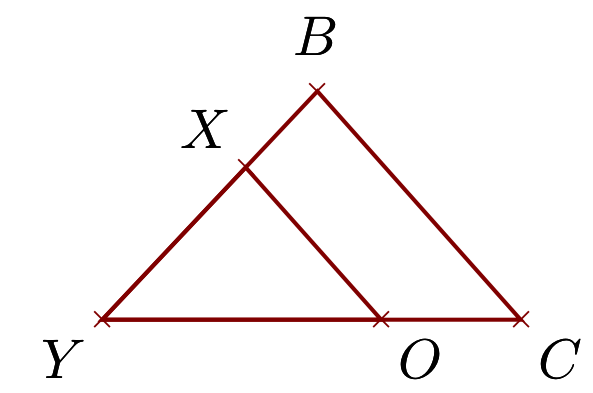
\includegraphics[width=0.4\linewidth]{3xx-dm/sources/dm2/tha1.png}
    \end{figure}

  \item[2.]Les droites (WM) et (VP) sont parallèles. \\
    On donne IW = 5 cm, W M = 3,7 cm, IP = 1,8 cm et V P = 2,5 cm.
    Calculer IM et IV .
    \begin{figure}[H]
      \centering
      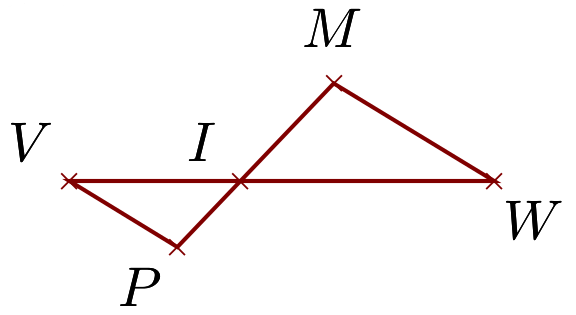
\includegraphics[width=0.4\linewidth]{3xx-dm/sources/dm2/tha2.png}
    \end{figure}

  \item[3.] On donne NK = 21 cm, PN = 8,4 cm, PQ = 13,2 cm et PL = 19,8 cm.\\
    Démontrer que les droites (KL) et (NQ) sont parallèles.
    \begin{figure}[H]
      \centering
      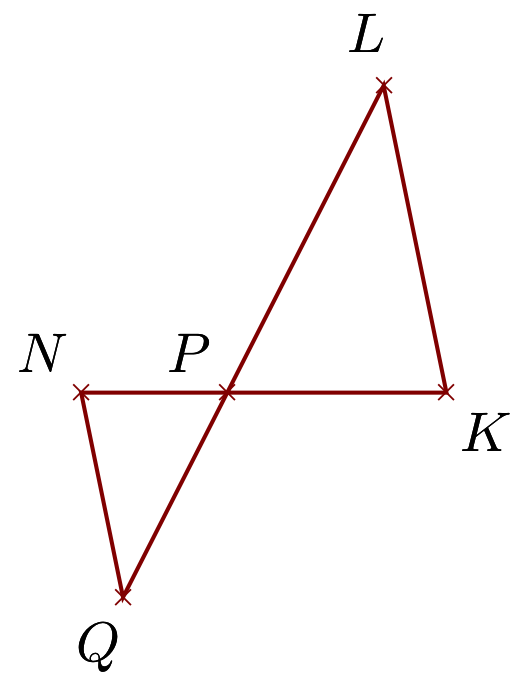
\includegraphics[width=0.4\linewidth]{3xx-dm/sources/dm2/tha3.png}
    \end{figure}
  \end{itemize}

\end{multicols}

\horrule{1px} 
\begin{multicols}{2}

  \subsection*{Ex - Résoudre}
  \textit{\textbf{Résoudre les équations.}}
  \begin{itemize}
  \item[1.] $2.5 \times 4 + b = 8 $
  \item[2.] $-5.6 \times 5 + b=  4.2 $
  \item[3.] $\dfrac{1}{2}\times 12 + b = 52 $
  \item[4.] $-15 \times 10 + b = 300 $
  \item[5.] $21 \times -4.8 + b = -80 $
  \item[6.] $32 \times -0.5 + b = -6 $
  \end{itemize}

\end{multicols}

\end{document}
